% ch10 —— 第 10 章 深谷賢治「ミラー対称性とホモロジー代数」
% 本章原书节号用阿拉伯数字（1, 2, …），而 preamble 默认 \thesection 为罗马数字。
% 章内局部改写为阿拉伯数字，章末再恢复（同 ch04，Lead 裁定 A 案）。
\renewcommand{\thesection}{\arabic{section}}
\chapter{镜像对称与同调代数}
\chapterauthor{深谷賢治}{[京都大学大学院理学研究科]}

% ===== PDF p.129 (原书 p.121) =====
\section{引言}

镜像对称猜想有一个与数学中其他有名有姓的猜想大不相同的地方。那就是：这个猜想并不是 well-defined 的。用更平常的话来说，镜像对称猜想的特征是，猜想本身的内容至今仍未确定。

一方面，这是个麻烦的地方：它很难登上“公平竞赛、比谁先解决问题”这个擂台，因为谁解决到了哪一步并不清楚。另一方面，也有人正因为如此，反而更喜欢镜像对称这类问题。

Candelas（P. Candelas）等人的那篇论文，使镜像对称在数学家中也广为人知。他们给出的，是 $\CP^4$ 中五次超曲面内有理曲线条数的计算方法。Candelas 等人的论证包含物理学的洞察，所以从数学的立场看，只能把它看作猜想。狭义上，人们把它称为镜像对称猜想。狭义意义的镜像对称猜想已由 Givental 等人解决。但是，我并不认为“镜像对称猜想”已经得到解决。

原本的镜像对称，被看作两个物理理论（场论）的一致。而“场论”在数学中还是一个尚未定义的概念。从关于场论的物理学洞察，可以得到各种不变量（等等）。两个物理理论一旦一致，就能得到它们的不变量之间的等式。这种等式的两边，在许多场合都可以给出数学上严格的定义；但其背后的场论，还没有成为数学。所以，把镜像对称猜想作为数学来表述，它就变成不变量之间的等式。五次超曲面内有理曲线的条数，与由某个复流形的周期所决定的量相一致；

% ===== PDF p.130 (原书 p.122) =====
Candelas 等人的这一结论，正属于由此得到的这一系列奇妙等式当中最早的几项之一。

用同样思路导出等式的工作，此后也做了很多。在 1990 年代的第二次弦理论革命中，又产生了更多并不包含在镜像对称范围之内的等式。这些等式同样可以通过抽取物理理论一致中能在数学上表述的部分而得到。进入 21 世纪后，这种情况依然在继续。

镜像对称猜想的最终主张之所以丝毫看不出会确定下来的迹象，有两个原因。其一，人们不断从中导出“数学的新等式”；其二，那些导出数学等式的物理洞察本身，至今仍无法作为数学上正确表述的猜想提出来。

\section{空间相等是什么意思}

如果放弃对镜像对称猜想作数学表述，则可以这样陈述。

\par\medskip
\noindent\textbf{对 Calabi--Yau 流形 $M$，存在称为其镜像的 Calabi--Yau 流形 $M'$。$M$ 上称为 A 模型的弦理论，与 $M'$ 上称为 B 模型的弦理论是等价的\footnote{在并非 Calabi--Yau 流形的场合，镜像对称性也正在被逐步推广。}。}
\par\medskip

A 模型、B 模型这些说法稍后再作说明。这里想说的，是两个弦理论等价这件事的含义。作为数学家，我对第 1 节所述镜像对称研究的现状非常不满。无论证明多少被预言的等式，不满都不会消除。因为若不经过数学上尚未得到正当化的物理洞察，就无法理解等式成立的理由与意义。理想的证明应当是：把弦理论在数学上准确地表述，给出从 $M$ 与 $M'$ 造出弦理论的 A、B 之类的处方，然后严格证明“弦理论”的同构，从而把这些等式一举导出。这次想讲的，是朝这个方向所作的尝试。

这里不处理“弦理论”是什么这个问题，而改为考虑：两个“弦理论”相等是什么意思。再把问题作如下
% ===== PDF p.131 (原书 p.123) =====
扩展。

\par\medskip
\noindent\textbf{两个“空间”相等是什么意思。}
\par\medskip

这个改写有几条背景。

（甲）镜像对称中的 $M$ 与 $M'$ 远比我们能直接观测的尺度小得多；我们能感知到它们，恐怕只能通过由它们间接呈现的各种量。

（乙）因此，下面两个命题没有区别：“$M$ 上称为 A 模型的弦理论与 $M'$ 上称为 B 模型的弦理论相等”；“空间 $M$ 等于空间 $M'$”。

在（乙）中我们说了“空间 $M$ 等于空间 $M'$”。但 $M$、$M'$ 是叫作 Calabi--Yau 流形的流形，一般会是彼此不同的流形。因此，相等的含义就与通常流形论中的含义不同。

再者，在某些场合，$M$ 这一边还是流形，$M'$ 却可能不再是流形，而变成别的东西。尤其是在把镜像对称推广到比 Calabi--Yau 流形更一般的情形时，就会如此。

镜像对称暗示着“空间”这一概念需要推广——其背景就在这里。

\section{层与拓扑斯}

把空间作为超出“点的集合”的东西来把握，这一方向昔日的推动者是 Grothendieck。本章的主题同调代数，也是 Grothendieck 为此使用的主要工具之一。要思考两个 Calabi--Yau 流形“相等”是什么意思，Grothendieck 的想法可供参考。

把空间一般化时，常被说到的一个想法，是把它换成“由空间上的函数构成的环”。

% ===== PDF p.132 (原书 p.124) =====
这样的想法。它被典型地用于被称为“非交换几何”的许多尝试之中\footnote{在弦理论的数学表述这一尝试之中，非交换几何也屡屡出现。}。概形（scheme）这一概念也用到这个想法。在与弦理论相关的数学的近期研究中，更一般化的“叠”（stack）之类也常常出现。

即使“函数的环”不同，实际上表示着同一个“空间”，这样的例子有环论中的现象——Morita 等价。下面说明它。考虑（含单位元 1 的）环 $R$，把以 $R$ 为系数的 $n\times n$ 矩阵全体记作 $M_n(R)$。下列主张是 Morita 等价的典型例子。

\par\medskip
\noindent\textbf{$R$ 上的模全体与 $M_n(R)$ 上的模全体之间，存在一一对应。}
\par\medskip

对 $R$ 上的模 $V$，考虑把 $V$ 并排 $n$ 个所得的模 $W = V^n = V\oplus\cdots\oplus V$。再在它上面如下给出 $M_n(R)$ 上的模结构。
“把 $V^n$ 的元看作竖向量，$M_n(R)$ 就能用普通的矩阵乘法来写。”
反之，考虑 $M_n(R)$ 上的模 $W$。设 $E_1$ 为只有 $1\times1$ 分量是 1、其余为 0 的矩阵。则 $V = \{E_1\cdot w \mid w \in W\}$ 成为 $R$ 上的模。

容易看出两个对应 $V \mapsto W$ 与 $W \mapsto V$ 互为逆对应，于是得到所求的对应。

以存在 Morita 等价为依据，人们认为 $R$ 所表示的“空间”与 $M_n(R)$ 所表示的“空间”是同一个。

模是对环而言确定的概念，而对更整体的对象，例如流形或概形，与模相对应的概念是层。

拓扑空间 $X$ 上的层，大体可以这样理解：对 $X$ 的开集 $U$，对应其上的“函数集合”$\mathcal{F}(U)$。对流形或概形，有被称为结构层的环的层。例如对流形 $M$，$C^\infty$ 函数的层 $C^\infty$ 就相当于它。$C^\infty$ 是对开集 $U\subset M$ 给出的对应：$U\mapsto U$ 上 $C^\infty$ 函数全体 $C^\infty(U)$。$C^\infty(U)$ 上定有加法与乘法，构成环，所以这是环的层。又，对于由方程

\[
  f_1(x_1,\dots,x_n) = 0,\quad \dots,\quad f_k(x_1,\dots,x_n) = 0
\]

确定的 $\C^n$ 的子集（仿射代数簇）$X$，环

\[
  R = \C[x_1,\dots,x_n]/(f_1,\dots,f_k)
\]

% ===== PDF p.133 (原书 p.125) =====
可以定义 $X$ 上的层 $\cO_X$。

所谓“对应于模”，是指这种结构层上的模的层。把 $R$-模这一概念大域化，就是 $\cO_X$-模的层这一概念。$\cO_X$-模的层的代表性例子，可以由 $X$ 上的向量丛，或者由 $X$ 的部分流形等作出来。它们成为被称为凝聚层的层。层与凝聚层这些概念的起源在多变数复函数论等之中，Leray 与岡潔奠定了其基础。经由 Henri Cartan 等 Bourbaki 学派的数学家，它被整理并引入数学的许多领域。同调代数这一领域，也是在那个时代与层的理论的诞生密切相关地发展起来的。Henri Cartan 与 Eilenberg、MacLane 一起是同调代数的建设者之一。

Serre 在 1950 年代写了“代数的凝聚层”这篇论文，在层的理论之下奠定了建立代数几何学的基础。把它发展下去，Grothendieck 的概形论就出现了。与此并行，小平邦彦等人以层的理论为基础，把复流形论作为独立于代数几何的领域建立了起来。

这样，层的想法在代数几何学与复流形论中，50 多年以前起就是主要想法。进一步，Grothendieck 在把空间概念从概形推广到拓扑斯时，用了如下想法。

\par\medskip
\noindent\textbf{空间就是其上能够考虑层的东西。}
\par\medskip

这样一来，点就从空间里消失了。也就是说，忘掉空间本身，只考虑其上的层（结构层上的凝聚层）\footnote{为避免误解，补充一句：在镜像对称中，确实使用“把空间换成其上的层的范畴”这一思想，但拓扑斯本身还不太被用到。}。

% ===== PDF p.134 (原书 p.126) =====
\section{导出范畴}

层（结构层上的凝聚层）构成范畴，成为所谓阿贝尔范畴。所谓范畴，就是“对象”（构成的“集合”）与两个对象之间“态射”构成的集合都已确定的东西。以层为对象、把两个层之间的态射取作它们之间的同态，这就是层的范畴。$\cO_X$-模的范畴在这里记作 $Sh(X)$。

$Sh(X)$ 的原型是环 $R$ 上的模的范畴。也就是说，以 $R$ 上的模为对象、以它们之间作为 $R$-模的同态为态射的范畴。例如，Morita 等价就是 $R$ 的模的范畴与 $M_n(R)$ 的模的范畴的同构（等价）。

我们把空间 $X$、特别是 Calabi--Yau 流形 $X$，换成其上的凝聚 $\cO_X$-模的范畴。这是在数学上表述“空间相等”时出现的重要想法，出现在 B 模型一侧。更详细地说，镜像对称中使用的不是范畴 $Sh(X)$，而是它的导出范畴。下面说明导出范畴。

同调代数的开端是同调群的定义。（据说是 Emmy Noether 提出的。）同调群由模的链复形 $(\{C_k\}_{k=0}^n, \{d_k\}_{k=1}^n)$ 定义。这里 $C_k$ 是模，$d_k : C_k \to C_{k-1}$ 是同态。$d_k$ 应满足的重要条件是

\[
  d_{k-1}\circ d_k = 0 \tag{1}
\]

这个等式，几何上对应于“集合的边界的边界是空集”这一事实。

链复形本来是为了定义同调群而引入的。同调群由两部分构成：$d_k x = 0$ 的 $x$ 全体 $\operatorname{Ker} d_k$，以及形如 $x = d_{k+1}y$ 的 $x$ 全体 $\operatorname{Im} d_{k+1}$。同调群就是前者对后者的商模。随着同调代数的发展，人们不再只用同调群，也开始用链复形本身来研究。让空间 $X$ 对应链复形 $S(X)$、考察其同调群，这就是同调论；而链复形 $S(X)$ 包含比同调群更多的信息。但链复形 $S(X)$ 并不是由空间 $X$ 唯一决定的。因此，要从链复形所持有的信息之中，取出不依赖于 $S(X)$ 的构造方式、而由空间 $X$

% ===== PDF p.135 (原书 p.127) =====
所决定的信息，就有必要这样做。

链复形的弱同构这个概念给出了这样的方法。在 $R$-模的链复形之间，可以确定一个叫弱等价的等价关系；以“$R$-模的链复形的弱等价类”为对象的范畴便确定下来。这个范畴称为“$R$-模范畴的导出范畴”。

% [Tutor Note: 原书把拟同构（quasi-isomorphism）称为「弱同构」，把导出范畴的对象称为「弱等价类」；以弱等价作局部化，正是导出范畴的标准造法。]

导出范畴对更一般的阿贝尔范畴也能作出来，特别地，$Sh(X)$ 的导出范畴 $\mathbb{D}(X)$ 就确定了。范畴 $\mathbb{D}(X)$ 在 B 模型的弦理论中起重要作用。也就是说，

\par\medskip
\noindent\textbf{$X$ 上 B 模型弦理论的 D-膜所构成的范畴，就是 $\mathbb{D}(X)$。}
\par\medskip

来说明这个命题。$\mathbb{D}(X)$ 的对象的例子，是 $X$ 上有两个向量丛 $E_1,E_2$，它们之间有同态 $\partial : E_1 \to E_0$ 这样的系统\footnote{在导出范畴里，本来应该用上同调而不是同调；但这里从同调讲起，就一路用同调讲下去。}。它的同调群是

\[
  H_1 = \operatorname{Ker}\partial \subset E_1
  \quad\text{与}\quad
  H_0 = \frac{E_0}{\operatorname{Im}\partial} .
\]

若 $\partial = 0$，则 $H_1 = E_1$、$H_0 = E_0$。若 $\partial \neq 0$，则 $H_k$ 变得比 $E_k$ 小。这件事可以看作 $\partial$ 把 $E_1,E_0$ 消去（cancel）掉一部分而使其变小。用导出范畴来解释 B 模型的 D-膜，似乎是 2000 年前后在物理学家之间才被理解的事情。

% [Tutor Note: 原书此处作「两个向量丛 $E_1,E_2$」，而映射写作 $\partial:E_1\to E_0$，下文同调群亦用 $E_0$；疑「$E_2$」为「$E_0$」之误，译文照录原文。]

范畴 $\mathbb{D}(X)$ 的重要性在数学中早就为人所知。例如，向井茂发现并深入研究过这样的现象。在环面或 $K3$ 曲面（两者都是 Calabi--Yau 流形的典型）上，即使 $X$ 与 $Y$ 不同，范畴 $\mathbb{D}(X)$ 与范畴 $\mathbb{D}(Y)$ 也会同构。这被视为“傅里叶变换的层论版本”，被称为傅里叶--向井变换。在与物理学的进展相互刺激之中，导出范畴 $\mathbb{D}(X)$ 的研究在代数几何中也兴盛起来。$\Pi$-稳定性是针对 $\mathbb{D}(X)$ 的对象定义的概念。它与 Kähler 结构模空间的关系、$\mathbb{D}(X)$ 与双有理几何的关系等，都在进展之中。

% ===== PDF p.136 (原书 p.128) =====
\section{A 模型与 B 模型}

我们说过，$X$ 上 B 模型弦理论的 D-膜所构成的范畴就是 $\mathbb{D}(X)$。下面再稍微谈一谈 B 模型与 A 模型。由于它们还没有作为数学得到定义，这里只叙述几个特征。

（a）B 模型的量由 $M$ 的复结构决定，A 模型的量由 $M$ 的辛结构决定。

（b）B 模型中许多量不受量子修正；A 模型的量则有量子修正。

说明一下上面用到的词。所谓 Calabi--Yau 流形，就是具有 Ricci 曲率为 0 的 Kähler 度量的复流形。流形的复结构，由把切向量映到切向量的对应 $J$（$J^2 = -1$）决定。（把它想成乘 $\sqrt{-1}$ 的映射也无妨。）给定 Riemann 度量 $g$ 与复结构 $J$，微分 2 形式 $\omega$ 由

\[
  \omega(X,Y) = g(X,JY) \tag{2}
\]

决定。（准确地说，微分 2 形式所应满足的条件 $\omega(X,Y) = -\omega(Y,X)$，在 $g$ 不是 $J$-不变时不成立。）微分 2 形式 $\omega$ 的外微分为 0 这个条件，就是度量是 Kähler 的条件。$\omega$ 决定辛结构。反之，若 $g$ 与 $\omega$ 满足某个相容性条件，则由 (2) 决定 $J$。

复流形或辛流形上，度量 $g$ 并不是事先定好的，所以复流形上并未定下辛结构，辛流形上也未定下复结构。A 模型的量只由辛结构决定，B 模型的量只由复结构决定——这就是（a）的主张\footnote{不过，随着把话题一般化下去，这一点会渐渐变得微妙。例如前一节提到的 $\Pi$-稳定性本是 B 模型的话题，却与 Calabi--Yau 流形的辛结构有关。}。

（b）与镜像对称研究的核心部分关系更深。前一节说过，层的理论自古就是复流形与代数簇研究的中心。在这个意义上，它们属于经典代数几何学与复几何学的范围。由此计算出来的量，是层系数上同调的各种
% ===== PDF p.137 (原书 p.129) =====
量，例如其同调群的秩，或者其上确定的结构的结构常数之类。这些都是经典的对象。在 B 模型的弦理论中，这类经典几何学的量直接作为弦理论的量出现，没有“量子修正”。还有一点很重要：出现的对象都是由局部地有意义的东西组装起来的。

层这个概念是局部的。设 $\mathcal{F}$ 是层。若 $\mathcal{F}(U)$ 的元 $s$ 在 $U$ 上各点的近旁都为 0，则 $s = 0$。又，层可以把局部的东西贴合成大域的东西。这就是局部性，是层的中心性质。我想这与“信息在空间中传播的速度有限”这一经典相对论量子力学的局部性也有关。这与（b）的主张，即 B 模型中没有量子修正这一主张，也有关。

另一方面，在第 6 节要说明的 A 模型中，没有那样的局部性。也就是说，A 模型的量不能通过对在空间上局部地确定的量作积分而得到。

不能用局部量的积分来表示的东西的典型例子，是出现在量子上同调环中的量子修正。量子上同调环是把普通上同调环的杯积作量子修正而得到的。用 de Rham 上同调表示，杯积的结构常数是积分

\[
  \int_{x\in M} u_1(x)\wedge u_2(x)\wedge u_3(x) \tag{3}
\]

所表示的。它成为 de Rham 上同调群 $H^*(M)$ 上的 3 次映射

\[
  H^*(M)\otimes H^*(M)\otimes H^*(M) \longrightarrow \R \tag{4}
\]

杯积的局部性，指的是积分 (3) 是在考虑 $u_1,u_2,u_3$ 在同一点 $x$ 处的值之下作出的。也就是说，这些“场”只在同一点之间才相互作用。

量子形变却不是这样。考虑从 $S^2$ 到 $M$ 的全纯（holomorphic）映射 $\varphi : S^2 \to M$，取其同调类 $\beta \in H_2(M)$。这类映射全体记作 $\cM_3(\beta)$。$\cM_3(\beta)$ 所给出的对杯积的量子修正，是
% ===== PDF p.138 (原书 p.130) =====
\[
  \mathcal{T}^{\,\beta\cap\omega}
  \int_{\varphi\in\cM_3(\beta)}
  u_1(\varphi(0))\wedge u_2(\varphi(1))\wedge u_3(\varphi(\infty))
\]

这样的积分。$\varphi(0),\varphi(1),\varphi(\infty)$ 是不同的点，所以这个“相互作用”发生在彼此分离的点之间。

% [Tutor Note: 原书 $\mathcal{T}$ 的指数印作 $\beta\cap\omega$；按上下文应理解为曲线类 $\beta$ 与 Kähler 形式 $\omega$ 的配对 $\int_\beta\omega$，即面积因子。]

这样，在 A 模型中局部性丧失了。所以 A 模型的量是关乎整个空间的大域量。五次超曲面内有理曲线的条数，就是其典型。局部量与整体（非局部）量相比，前者计算更容易。镜像对称的威力，就在于把 A 模型中出现的非局部量归结为 B 模型中的局部计算。

\section{Floer 同调与同调镜像对称}

第 5 节中，我们作为 A 模型中出现的典型量，考虑了量子杯积的结构常数。这是 Candelas 等人所考虑的量，对应有理曲线的条数。如第 4 节所述，我们把 B 模型的“空间”换成了其上的层所构成的范畴 $Sh(M')$，或它的导出范畴 $\mathbb{D}(M')$。这个范畴 $Sh(M')$ 在 A 模型中的对应物，是由 $M$ 上的 Floer 同调定出的范畴 $Lag(M)$。这就是 Kontsevich 的同调镜像对称猜想。范畴的一致（同构）与数的一致相比是精细得多的主张；借助它可以接近“空间相等”这一原本的镜像对称主张。

说明一下 A 模型一侧的范畴 $Lag(M)$。前面说过，B 模型一侧的范畴 $\mathbb{D}(M')$ 的对象是 D-膜。在 B 模型一侧，其理由不太容易看清；A 模型一侧则更明快。

D-膜是什么？它是作为弦的边界条件而出现的东西。顺便说一句，D 是 Dirichlet 的首字母，名字来源于 Dirichlet 边界条件。例如，对圆盘 $D^2 = \{(x,y)\mid x^2+y^2<1\}$ 上的函数 $f$，考虑 Laplace 方程 $\Delta f = 0$。这时指定 $f$ 在边界 $S^1 = \{(x,y)\mid x^2+y^2=1\}$ 上的值 $f(\cos\theta,\sin\theta)$，这就是 Dirichlet 边界条件。

弦理论的主角是弦，也就是绳。绳随时间运动留下的轨迹成为曲面 $\Sigma$。因此，流形 $M$ 中绳的轨迹是
% ===== PDF p.139 (原书 p.131) =====
$\varphi : \Sigma \to M$ 这样的映射。当弦是开的，即不是圆周而是区间时，$\Sigma$ 就有边界。也就是说，要考虑从带边界的曲面 $\Sigma$ 出发的映射 $\varphi : \Sigma \to M$。

映射 $\varphi$ 应满足的方程就是弦的运动方程。在所谓拓扑弦（topological string）这种（简单的）情形下，它就是“$\varphi$ 成为全纯映射”这个方程。换句话说，Cauchy--Riemann 方程就是运动方程。

Cauchy--Riemann 方程是椭圆型方程。在带边界的流形（这里是曲面）上考虑椭圆型方程时，需要边界条件。第 5 节出现的 $\cM_3(\beta)$ 是从 $S^2$ 出发的全纯映射的空间。把它换成从 $S^2$ 以外、带边界的 Riemann 面出发的全纯映射，就得到考虑 D-膜时由 A 模型得到的量。

$\cM_3(\beta)$ 是有限维空间。只要边界条件取得好，从带边界的 Riemann 面出发的全纯映射的空间也是有限维的。适当的边界条件是

\[
  \varphi(S^1) \subset L \tag{5}
\]

这个条件，即 Dirichlet 边界条件。$L$ 是 $\dim M/2$ 维的流形；进一步，还需要“全实，即 $L$ 的切空间不含复向量空间”这个条件。（没有这个条件，方程会在边界处退化，无法很好地作出解的模空间。）不过，作为 D-膜起作用的，是比“全实”更强的“Lagrangian 子流形”这一条件。

前面写过，A 模型中辛结构是主角。所谓辛结构，就是微分 2 形式 $\omega$ 满足 $d\omega = 0$，并且 $\omega$ 在每点非退化。在 $2n$ 维辛流形 $M$ 中，$n$ 维子流形 $L$ 是 Lagrangian 子流形，是指 $\omega$ 限制到 $L$ 上时变为 0。取 Lagrangian 子流形 $L$，考虑满足边界条件 (5) 的 $\varphi$。这时积分 $\int\varphi^*\omega$ 在 $\varphi$ 的连续形变下不变。

第 8 章说明 Floer 同调时，考虑了环路空间 $\Omega(M)$，即 $S^1 \to M$ 的映射，并考虑其上的泛函的极值问题。那时也说过，其隧道效应与量子上同调有关。

% ===== PDF p.140 (原书 p.132) =====
在本节所考虑的 D-膜存在的情形下，要把 $\Omega(M)$ 稍作替换。也就是说，考虑两个 Lagrangian 子流形（即 D-膜）$L_0,L_1$，并考虑

\[
  \Omega(L_0,L_1) = \{ l : [0,1]\to M \mid l(0) = L_0,\ l(1) = L_1 \} .
\]

这就是考虑从 $L_0$ 出发、在 $L_1$ 结束的弦。在这上面考虑 Morse 理论，但所用的泛函 $\mathcal{A}$ 如下。设 $l, l' \in \Omega(L_0,L_1)$。考虑连结这两者的 $\Omega(L_0,L_1)$ 中的道路 $\gamma(s)$，即满足 $\gamma(s) \in \Omega(L_0,L_1)$、$\gamma(0) = l$、$\gamma(1) = l'$ 的 $\gamma$。这时得到映射 $\varphi^\gamma : [0,1]\times[0,1]\to M$，它由

\[
  \varphi^\gamma(s,t) = \gamma(s)(t)
\]

给出。（$\gamma(s)$ 曾是 $[0,1]\to M$ 的映射，右边就是把它代入 $t$ 所得的东西。）泛函 $\mathcal{A}$ 这样取：

\[
  \mathcal{A}(l') - \mathcal{A}(l)
  = \int_{[0,1]\times[0,1]} \varphi^{\gamma*}\omega .
\]

（实际上这样的 $\mathcal{A}$ 不是单值函数，而是多值的。）

展开关于泛函 $\mathcal{A}$ 的 Morse 理论。由此定义出来的，就是两个 Lagrangian 子流形之组的 Floer 同调 $HF(L_0,L_1)$。

在没有“量子修正”的场合，它成为对每个交点 $p \in L_0\cap L_1$ 都有一个基底的 $\Q$ 向量空间。这是因为 $\mathcal{A}$ 的临界点对应于 $p \in L_0\cap L_1$ 的 $l_p(t) \equiv p$。

但实际上有量子修正。量子修正由图 1 所示那样的全纯映射 $D^2 \to M$ 给出。

所谓范畴 $Lag(M)$，大体上是这样一个范畴：以 Lagrangian 子流形 $L$ 为对象，从 $L_0$ 到 $L_1$ 的态射全体构成的集合为 Floer 同调 $HF(L_0,L_1)$。定义范畴所必需的态射的合成：

\[
  HF(L_0,L_1)\otimes HF(L_1,L_2) \longrightarrow HF(L_0,L_2) \tag{6}
\]

是借助图 2 那样的全纯三角形来定义的\footnote{其实刚写在这里的说法并不准确，需要作各种修正。关于这一点，第 8 节会稍微提到。}。Kontsevich 的同调镜像对称猜想是

\[
  \mathbb{D}(M') \cong \mathbb{D}(Lag(M)) \tag{7}
\]

右边是范畴 $Lag(M)$ 的导出范畴。

这个猜想目前对 2 维环面（椭圆曲线）已完全解决；

% ===== PDF p.141 (原书 p.133) =====
\begin{center}
  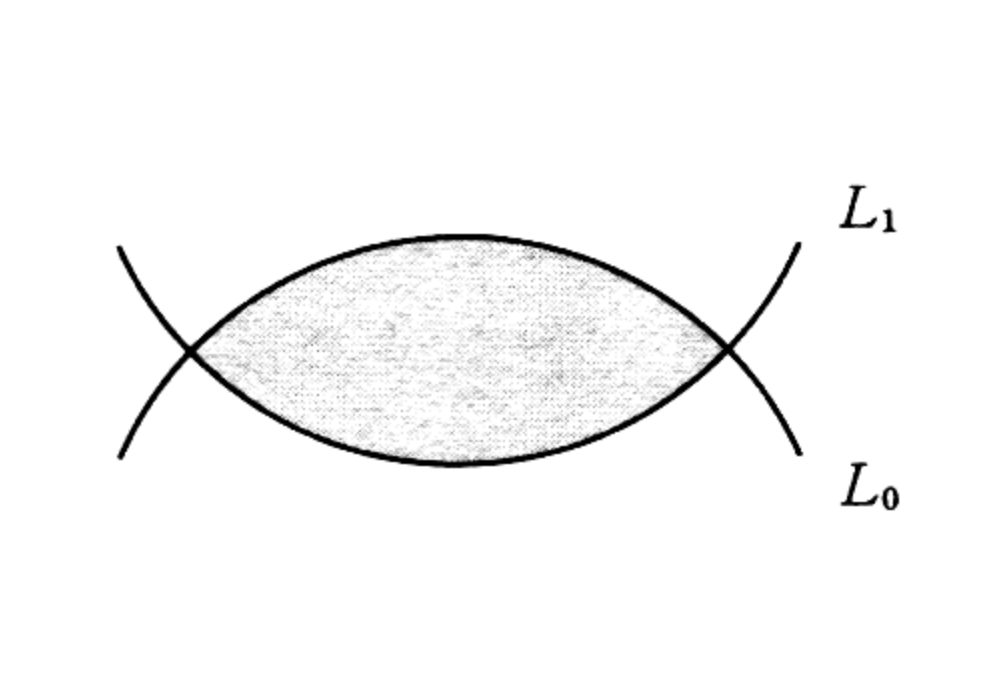
\includegraphics[width=0.56\linewidth]{figures/ch10-fig1.png}
\end{center}
\figtitle{1}{边界落在 $L_0,L_1$ 上的全纯圆盘（阴影部分）；量子修正由图 1 所示的这类全纯映射 $D^2\to M$ 计数得到（原书 p.133）}

\begin{center}
  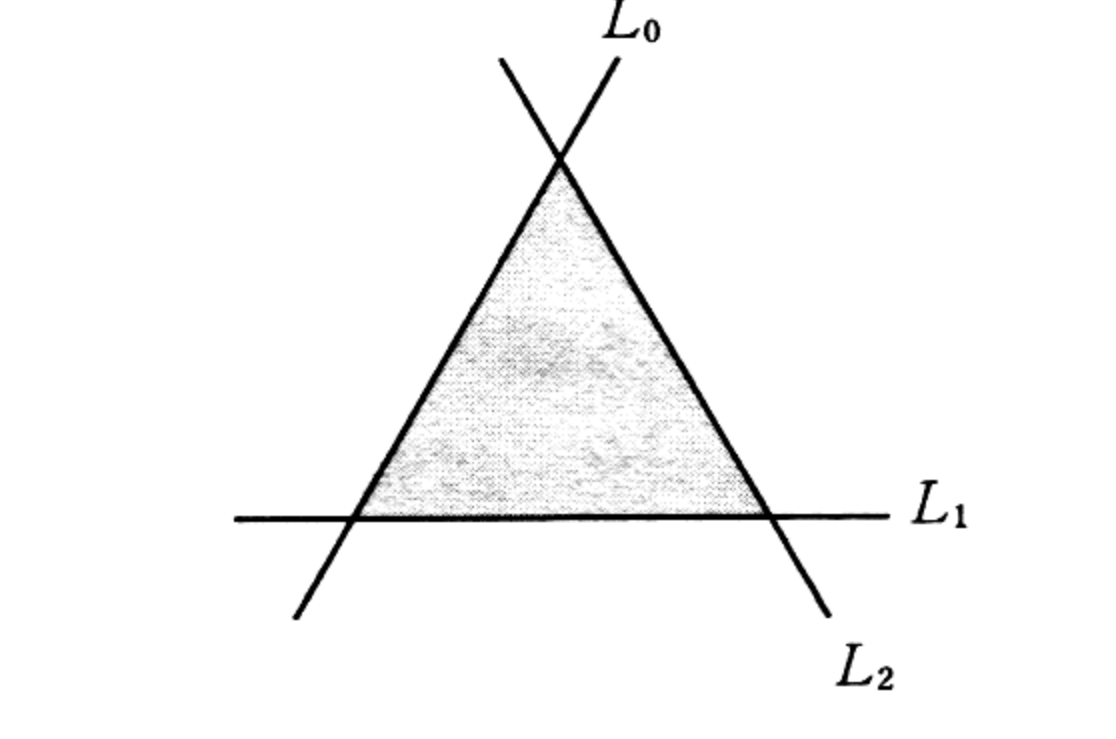
\includegraphics[width=0.56\linewidth]{figures/ch10-fig2.png}
\end{center}
\figtitle{2}{由 $L_0,L_1,L_2$ 围成的全纯三角形（阴影部分）；态射的合成 (6) 借助这种全纯三角形来定义（原书 p.133）}

% [Tutor Note: 原书此页两幅图以「図 1」「図 2」标识，本译本的图号与题注为译者所加。图 1 的阴影表示以 $L_0,L_1$ 的弧为边界的全纯圆盘；图 2 的阴影表示由 $L_0,L_1,L_2$ 围成的全纯三角形。]

高维环面则已部分解决，3 维射影空间中的 4 次曲面也已完全解决。这些都是 Calabi--Yau 流形的情形；在它们的推广中，还有各种各样已被解决的情形。据说 Kontsevich 最初（1993 年）提出这个猜想时，曾称之为“科幻（science fiction）”。而现在通往解决的道路已相当可见。

笔者与 Oh、太田、小野三人做了大约 10 年的工作，其中一项应用是范畴 $Lag(M)$ 的严格定义。这一部分已在 2006 年完成，可以说直到那时，同调镜像对称猜想 (7) 才成为数学的猜想。

\section{不变量的范畴化}

Floer 同调，应当说是“相交数的群化”。也就是说，它是这样一种同调论：取其所含秩的交错和，就得到相交数。把 Floer 同调纳入其中的范畴 $Lag(M)$，更应当说是相交数的范畴化（categorification）。

不变量的范畴化近来做出了各种东西。有名的有纽结或 3 维流形量子不变量的范畴化，即 Khovanov 同调等。

% ===== PDF p.142 (原书 p.134) =====
不变量范畴化之始，是 Segal 对共形场论的表述。Segal 把共形场论定义为从某个范畴出发的函子。那个范畴，是以 $S^1$ 的有限个不交并为对象、以它们之间以这些 $S^1$ 为边界的 Riemann 面为态射的范畴。

Floer 同调中有规范理论的东西，也有关于辛流形的东西。规范理论的 Floer 同调，对 3 维流形对应一个群。它与 4 维流形的 Donaldson 不变量有密切关系。要把这个 4 维--3 维规范理论的关系推广到 2 维，就有必要考虑带边界的 3 维流形 $M$ 的 Floer 同调。1992 年在 Warwick 大学的研讨会演讲中，Donaldson 画了与图 2 相同的图。他说道：带边界的 3 维流形的 Floer 同调，第一近似就是考虑这样的范畴。其中出现的辛流形，是由作为 $M$ 的边界的 2 维流形上的平坦联络所构成的流形。

听到这番话，笔者注意到：只要把范畴推广为 $A_\infty$ 范畴这一概念，带边界的 3 维流形的 Floer 同调就可以看作从那个范畴出发的函子。这件事于 1993 年在谷口研讨会上发表。听到它的 Kontsevich 由此到达了同调镜像对称猜想 (7)，并在当年的马克斯·普朗克研究所年会上发表。

关于带边界的 3 维流形 Floer 同调的根本问题，当时的构想至今尚未实现。最近终于出现了可能实现的征兆。把规范理论从 2 维到 4 维累积起来这一构想本身，以稍有不同、但被认为与 Seiberg--Witten 理论一致的形式实现了。这就是 Ozsváth--Szabó 的 Heegaard Floer 理论。

\section{同调代数与场论}

范畴 $Lag(M)$ 不应看作普通的范畴，而应看作 $A_\infty$ 范畴。不这样做，同调镜像对称猜想就不能成立。这个
% ===== PDF p.143 (原书 p.135) =====
$A_\infty$ 的 A，是结合（Associative）的首字母。范畴中决定性的重要结构是态射的合成 (6)。态射的合成满足结合律

\[
  (f\circ g)\circ h = f\circ(g\circ h) \tag{8}
\]

能把范畴看作群的推广，理由就是这种合成的结合性。再者，这里所考虑的范畴中，态射的集合上定义了加法，所以也可以看作环的推广。合成 (6) 的结构常数，成了量子上同调环的结构常数在存在 D-膜时的类似物。

说明导出范畴时写过：从链复形移到同调，信息就会丢失。范畴 $Lag(M)$ 的情形也一样：若把态射的集合做成同调群 $HF(L_0,L_1)$，重要信息就会丢失。把范畴 $Lag(M)$ 作为“空间”的替代物使用时，必须保留那些一旦取同调就会丢失的信息。为了不取同调群、而按链复形原样处理其种种结构，就需要同调代数。这样的同调代数，从 1970 年代以前起就在代数拓扑等领域被大量研究。带有结构的链复形的同调代数对场论研究是必要的——这一点逐步明确起来，是 1980 年代后半到 1990 年代前半的事。Witten 在 80 年代后半讲述了非交换几何与弦理论的关系，那里出现了 $A_\infty$ 代数。Zwiebach 在 90 年代研究了开弦场论（string field theory），那里也出现了与链复形的同调代数同样的考察。

Floer 同调之间的积结构，作为 $A_\infty$ 代数或 $A_\infty$ 范畴来表述，才是正确的做法。一般情形的 Floer 同调，为了定义它，必须把 $A_\infty$ 结构考虑进去。这是由于在一般 Floer 同调中式 (1) 不成立这一现象（BRST 反常）造成的。

% [Tutor Note: BRST 反常（anomaly）指经典对称性在量子化后不能保持的现象；此处指（1）式 $d_{k-1}\circ d_k=0$ 在一般 Floer 同调中只能在高阶（$A_\infty$）意义下成立。]

$A_\infty$ 结构只涉及开 Riemann 面中的圆盘，只对应开弦理论的一部分。处理一般开弦的同调代数框架，目前正在被搭建起来，但尚未完成。

最后，说明一下 $A_\infty$ 代数这类高阶积结构出现的理由，以此结束本章。

进入同调群的积结构是杯积的近亲。杯积按 (4) 那样
% ===== PDF p.144 (原书 p.136) =====
重新理解，就对应 3 次函数。要读出全部信息，就必须考虑 4 次、5 次……所有次数的函数。即使原本链复形上的结构只到 3 次（即只到积结构），一旦要把信息塞进同调群，4 次以上的项也会进来。

这可以这样说明。同调群对应质量为 0 的粒子，它们之间的积结构表示相互作用。质量为 0 的粒子之间的相互作用中，可能出现质量为正的粒子作为中间状态。要把“积结构塞进同调”，就必须让中间状态的效应进入同调上的积结构。这是物理学中所谓重整化（renormalization）的操作之一；其结果，原本只到 3 次的相互作用中会出现高阶项。

% [Tutor Note: 重整化在这里指把中间状态（高能自由度）的效应吸收进低能有效理论的做法；正是它把原本只到 3 次的积结构提升为含 4 次以上高阶项的 $A_\infty$ 结构。]

对应于没有环（loop）的图的效果，就是 $A_\infty$ 代数（按对称性的种类，还会出现 $L_\infty$ 代数等其他结构）。若把有环的情形也包括进来，它应当成为这样一个代数结构：用同调代数给出从一般 Riemann 面出发的映射之效应的表述。

% [Tutor Note: 原书本章末尾附有作者姓名的假名读音标记，译文按全书体例省略；作者名已在章首署名中给出。]

% 本章节号恢复为全书默认的罗马数字（章内曾临时改为阿拉伯数字以照应原书）。
\renewcommand{\thesection}{\Roman{section}}
